\documentclass[tikz,border=6pt]{standalone}
\usepackage{pgfplots}
\pgfplotsset{compat=1.18}
\usepgfplotslibrary{colormaps}
\usetikzlibrary{arrows, arrows.meta, calc}
\usetikzlibrary{decorations.markings}


\usepackage{amssymb,amsmath,mathtools}

\usepackage[T1]{fontenc}
\usepackage[utf8]{inputenc}
\usepackage{newpxtext,newpxmath}
\usepackage{sectsty}

\renewcommand{\Re}{\operatorname{\mathrm{Re}}}
\renewcommand{\Im}{\operatorname{\mathrm{Im}}}

\begin{document}
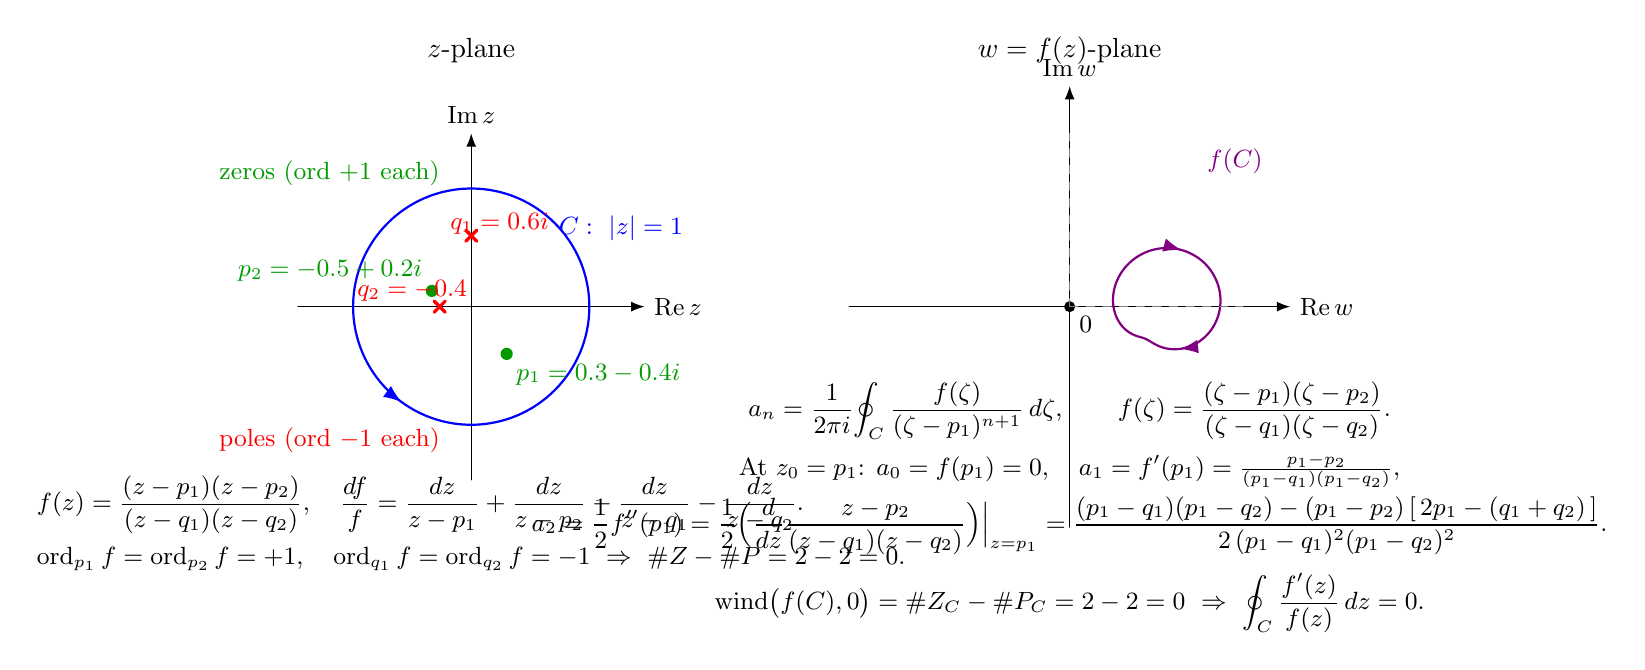
\begin{tikzpicture}[>=Latex, line cap=round, line join=round, font=\small]

%========================
% Left: z-plane
%========================
\begin{scope}[shift={(0,0)}]
	\node[font=\normalsize] at (0,3.25) {$z$-plane};
	% axes
	\draw[->] (-2.2,0)--(2.2,0) node[right] {$\Re z$};
	\draw[->] (0,-2.2)--(0,2.2) node[above] {$\Im z$};
	
	% unit circle C (positively oriented) -- radius 1.5 for visibility
	\draw[blue,thick,postaction={decorate},
	decoration={markings, mark=at position 0.65 with {\arrow{>}}}]
	(0,0) circle (1.5);
	\node[blue] at (1.9,1.0) {$C:\ |z|=1$};
	
	% zeros at p1, p2 (order +1 each)
	\fill[green!60!black] (0.45,-0.60) circle(2.2pt) node[below right] {$p_1=0.3-0.4i$};
	\fill[green!60!black] (-0.50,0.20) circle(2.2pt) node[above left] {$p_2=-0.5+0.2i$};
	\node[green!60!black] at (-1.8,1.7) {zeros (ord $+1$ each)};
	
	% poles at q1, q2 (order -1 each)
	\draw[red,very thick] (0,0.90) ++(-0.07,-0.07) -- ++(0.14,0.14);
	\draw[red,very thick] (0,0.90) ++(-0.07,0.07)  -- ++(0.14,-0.14);
	\node[red] at (0.36,1.05) {$q_1=0.6i$};
	\draw[red,very thick] (-0.40,0) ++(-0.07,-0.07) -- ++(0.14,0.14);
	\draw[red,very thick] (-0.40,0) ++(-0.07,0.07)  -- ++(0.14,-0.14);
	\node[red] at (-0.75,0.2) {$q_2=-0.4$};
	\node[red] at (-1.8,-1.7) {poles (ord $-1$ each)};
	
	% function label + orders via the winding/log-derivative form
	\node[align=left] at (0,-2.75) {$\displaystyle
		f(z)=\frac{(z-p_1)(z-p_2)}{(z-q_1)(z-q_2)},\quad
		\frac{df}{f}=\frac{dz}{z-p_1}+\frac{dz}{z-p_2}-\frac{dz}{z-q_1}-\frac{dz}{z-q_2}.
		$\\[4pt]
		$\displaystyle
		\operatorname{ord}_{p_1}f=\operatorname{ord}_{p_2}f=+1,\quad
		\operatorname{ord}_{q_1}f=\operatorname{ord}_{q_2}f=-1
		\ \Rightarrow\ \#Z-\#P=2-2=0.$};
\end{scope}

%========================
% Right: w-plane = f(z)-plane
%========================
\begin{scope}[shift={(7.6,0)}]
	\node[font=\normalsize] at (0,3.25) {$w=f(z)$-plane};
	% axes
	\draw[->] (-2.8,0)--(2.8,0) node[right] {$\Re w$};
	\draw[->] (0,-2.8)--(0,2.8) node[above] {$\Im w$};
	
	% origin
	\fill (0,0) circle(2pt) node[below right] {$0$};
	
	% image curve f(C): z = x+iy = 1.5 e^{it} -> w = (z-p1)(z-p2)/[(z-q1)(z-q2)]
	% Concrete parameters (match left):
	% p1=(0.3,-0.4), p2=(-0.5,0.2), q1=(0,0.6), q2=(-0.4,0)
	% Define helpers:
	%   u1 = x-0.3, v1 = y+0.4
	%   u2 = x+0.5, v2 = y-0.2
	%   a  = x,     b  = y-0.6
	%   c  = x+0.4, d  = y
	% N = (u1+iv1)(u2+iv2) = (ReN)+i(ImN)
	% D = (a+ib)(c+id)     = (ReD)+i(ImD)
	% Re w = (ReN ReD + ImN ImD)/den,  Im w = (ImN ReD - ReN ImD)/den,  den=ReD^2+ImD^2
	\draw[violet,thick,
	postaction={decorate},
	decoration={markings,
		mark=at position 0.20 with {\arrow{>}},
		mark=at position 0.62 with {\arrow{>}}}]
	plot[domain=0:6.283, samples=720]
	({
		% Re w
		(
		% ReN*ReD
		( (1.5*cos(\x r)-0.3)*(1.5*cos(\x r)+0.5) - (1.5*sin(\x r)+0.4)*(1.5*sin(\x r)-0.2) )
		*
		( (1.5*cos(\x r))*(1.5*cos(\x r)+0.4) - (1.5*sin(\x r)-0.6)*(1.5*sin(\x r)) )
		+
		% ImN*ImD
		( (1.5*cos(\x r)-0.3)*(1.5*sin(\x r)-0.2) + (1.5*cos(\x r)+0.5)*(1.5*sin(\x r)+0.4) )
		*
		( (1.5*cos(\x r))*(1.5*sin(\x r)) + (1.5*sin(\x r)-0.6)*(1.5*cos(\x r)+0.4) )
		)
		/
		(
		% den
		( (1.5*cos(\x r))*(1.5*cos(\x r)+0.4) - (1.5*sin(\x r)-0.6)*(1.5*sin(\x r)) )^(2)
		+
		( (1.5*cos(\x r))*(1.5*sin(\x r)) + (1.5*sin(\x r)-0.6)*(1.5*cos(\x r)+0.4) )^(2)
		)
	},
	{
		% Im w
		(
		% ImN*ReD
		( (1.5*cos(\x r)-0.3)*(1.5*sin(\x r)-0.2) + (1.5*cos(\x r)+0.5)*(1.5*sin(\x r)+0.4) )
		*
		( (1.5*cos(\x r))*(1.5*cos(\x r)+0.4) - (1.5*sin(\x r)-0.6)*(1.5*sin(\x r)) )
		-
		% ReN*ImD
		( (1.5*cos(\x r)-0.3)*(1.5*cos(\x r)+0.5) - (1.5*sin(\x r)+0.4)*(1.5*sin(\x r)-0.2) )
		*
		( (1.5*cos(\x r))*(1.5*sin(\x r)) + (1.5*sin(\x r)-0.6)*(1.5*cos(\x r)+0.4) )
		)
		/
		(
		( (1.5*cos(\x r))*(1.5*cos(\x r)+0.4) - (1.5*sin(\x r)-0.6)*(1.5*sin(\x r)) )^(2)
		+
		( (1.5*cos(\x r))*(1.5*sin(\x r)) + (1.5*sin(\x r)-0.6)*(1.5*cos(\x r)+0.4) )^(2)
		)
	});
	\node[violet] at (2.1,1.85) {$f(C)$};
	
	% dashed rays to visualize winding (here: 0)
	\draw[gray,dashed] (0,0) -- (2.2,0);
	\draw[gray,dashed] (0,0) -- (0,2.2);
	
	% annotation: Taylor coefficients at z_0 = p_1 via Cauchy integrals
	\node[align=center] at (0,-2.55)
	{$\displaystyle
		a_n=\frac{1}{2\pi i}\!\oint_C \frac{f(\zeta)}{(\zeta-p_1)^{n+1}}\,d\zeta,\qquad
		f(\zeta)=\frac{(\zeta-p_1)(\zeta-p_2)}{(\zeta-q_1)(\zeta-q_2)}.$\\[4pt]
		At $z_0=p_1$: $a_0=f(p_1)=0,\quad
		a_1=f'(p_1)=\frac{p_1-p_2}{(p_1-q_1)(p_1-q_2)},$\\[2pt]
		$\displaystyle
		a_2=\frac{1}{2}f''(p_1)=\frac{1}{2}\Big(\frac{d}{dz}\frac{z-p_2}{(z-q_1)(z-q_2)}\Big)\Big|_{z=p_1}
		=\frac{(p_1-q_1)(p_1-q_2)-(p_1-p_2)\,[\,2p_1-(q_1+q_2)\,]}{2\,(p_1-q_1)^{2}(p_1-q_2)^{2}}.$\\[6pt]
		$\mathrm{wind}\big(f(C),0\big)=\#Z_C-\#P_C=2-2=0
		\ \Rightarrow\
		\displaystyle \oint_C \frac{f'(z)}{f(z)}\,dz=0.$};
\end{scope}

\end{tikzpicture}
\end{document}